\documentclass[10pt,a4paper]{article}
\usepackage[utf8]{inputenc}
\usepackage[T1]{fontenc}
\usepackage{lmodern}
\usepackage[margin=1.2cm]{geometry}
\usepackage{booktabs}
\usepackage{amsmath,amssymb}
\usepackage{graphicx}
\usepackage{setspace}
\usepackage{caption}
\usepackage{subcaption}
\usepackage{xcolor}
\usepackage{hyperref}
\usepackage{float}

\setlength{\parskip}{2pt}
\setlength{\itemsep}{0pt}
\setlength{\floatsep}{6pt plus 2pt minus 2pt}
\setlength{\textfloatsep}{8pt plus 2pt minus 2pt}
\setlength{\intextsep}{6pt plus 2pt minus 2pt}

\captionsetup{skip=3pt}

\hypersetup{
    colorlinks=true,
    linkcolor=blue!70!black,
    citecolor=blue!70!black,
    urlcolor=blue!70!black
}

\definecolor{headerblue}{RGB}{20, 40, 70}

\begin{document}

% =============================================================================
% PAGINA 1: MODELLO BASELINE, TEST DI CHOW E CONFRONTO ORACOLO
% =============================================================================
\noindent {\LARGE \textbf{\color{headerblue}Analisi Comparativa del Detrending: Baseline vs Full-Sample}}
\vspace{0.35em}
\hrule height 0.8pt
\vspace{0.45em}

% -----------------------------------------------------------------------------
% 1. SCELTA DEL DETRENDING BASELINE
% -----------------------------------------------------------------------------
\noindent \textbf{\large 1. Scelta del modello di detrending baseline}
\vspace{0.15em}

\noindent Per rimuovere la componente tecnologica secolare ho adottato un \textbf{trend lineare OLS stimato per ciascuna contea in expanding window} (finestra iniziale 1951--1980 e aggiornamento causale anno per anno $t < Y$). Tra i modelli candidati (Tabella~\ref{tab:thesis_detrending_comp}), la specificazione lineare minimizza l'errore fuori campione ($5.77$\,bu/ac su $4{,}050$ stime OOS a 1 passo nel periodo pre-test 1981--2010), \`e selezionata dal BIC nel $65.9\%$ delle contee ed evita le oscillazioni ai bordi tipiche delle forme polinomiali. Per prevenire look-ahead bias sul test set dei modelli (2011--2025), la selezione del detrending \`e condotta esclusivamente sul periodo pre-test. Sull'intero campione 1951--2025, il \textbf{polinomio cubico} registra invece il maggior $R^2$ in-sample ($0.831$ a livello di contea e $0.943$ aggregato), motivo per cui viene impiegato come controllo di robustezza. La stima tramite media mobile dell'incremento annuo richiede finestre ampie ($27$ anni) per non interpretare le siccit\`a estreme (1983 e 1988) come flessioni permanenti del trend.

\begin{table}[H]
\centering
\singlespacing
\scriptsize
\setlength{\tabcolsep}{3.5pt}
\renewcommand{\arraystretch}{1.06}
\caption{Confronto tra specificazioni di detrending candidate: bont\`a di fit ($R^2$, 1951--2025) ed errore OOS pre-test (1981--2010).}
\label{tab:thesis_detrending_comp}
\begin{tabular*}{\textwidth}{@{\extracolsep{\fill}} l c ccc ccc @{}}
\toprule
& & \multicolumn{3}{c}{\textbf{Aggregato Regionale ($N=75$)}} & \multicolumn{3}{c}{\textbf{Livello di Contea ($135$ contee)}} \\
\cmidrule(lr){3-5}\cmidrule(lr){6-8}
\textbf{Specificazione} & \textbf{Parametri ($k$)} & \textbf{$R^2$} & \textbf{RSE (bu/ac)} & \textbf{RMSE OOS} & \textbf{$R^2$} & \textbf{RMSE OOS (bu/ac)} & \textbf{\% BIC Favorito} \\
\midrule
\textbf{Lineare OLS (Baseline)} & 2 & 0.932 & 2.87 & \textbf{3.28} & 0.812 & \textbf{5.77} & \textbf{65.9\%} \\
Quadratico & 3 & 0.940 & 2.72 & 3.51 & 0.825 & 6.14 & 24.4\% \\
Cubico (Miglior In-Sample) & 4 & \textbf{0.943} & \textbf{2.67} & 3.84 & \textbf{0.831} & 6.62 & 9.7\% \\
\bottomrule
\end{tabular*}
\vspace{0.2em}
{\scriptsize\textit{Note:} $R^2$, RSE e \% BIC calcolati sull'intero campione storico 1951--2025 ($10{,}125$ osservazioni). L'RMSE OOS \`e stimato a 1 passo in expanding window sul solo periodo pre-test 1981--2010 ($4{,}050$ previsioni fuori campione) per escludere il test set 2011--2025 dalla selezione del modello di detrending.}
\end{table}

\vspace{0.2em}
% -----------------------------------------------------------------------------
% 2. TEST DI CHOW SUI BREAK STRUTTURALI E CONFRONTO ORACOLO
% -----------------------------------------------------------------------------
\noindent \textbf{\large 2. Test di Chow sui break strutturali e confronto con il trend totale}
\vspace{0.15em}

\noindent Un'ipotesi aperta riguarda l'eventuale accelerazione del progresso tecnico nel quindicennio recente (2011--2025), dove la stima in expanding window potrebbe scontare un'inerzia legata ai primi decenni del campione.

\noindent Il \textbf{test di Chow sui break strutturali} applicato alla serie storica aggregata (1951--2025) individua un punto di rottura significativo nel \textbf{2014}: la statistica $F$ raggiunge $F = 21.96$ per il salto di livello ($p < 0.0001$, incremento medio stimato di $\boldsymbol{+4.83}$\,bu/ac, $\Delta\text{BIC} = -15.64$; Figura~\ref{fig:chow_break}). Il cambio di pendenza non risulta significativo ($p = 0.74$). Poich\'e tale break emerge a posteriori sull'intero campione, un'eventuale modellazione endogena del cambio di regime nella tesi andrebbe validata causalmente sul periodo pre-test per evitare look-ahead bias.

\noindent Per verificare se questo ritardo o una flessibilit\`a non lineare alterino la contrazione dei modelli nelle annate avverse ($D_1$), ho ricalcolato l'intera pipeline predittiva adottando come controllo di robustezza il \textbf{trend polinomiale cubico a livello di singola contea stimato sull'intero periodo 1951--2025 ($R^2 = 0.831$ di contea, $0.943$ aggregato)}. Questa specificazione incorpora l'informazione dell'intero campione e costituisce il benchmark oracolo per isolare il ruolo del trend da quello delle variabili meteorologiche.

\begin{figure}[H]
    \centering
    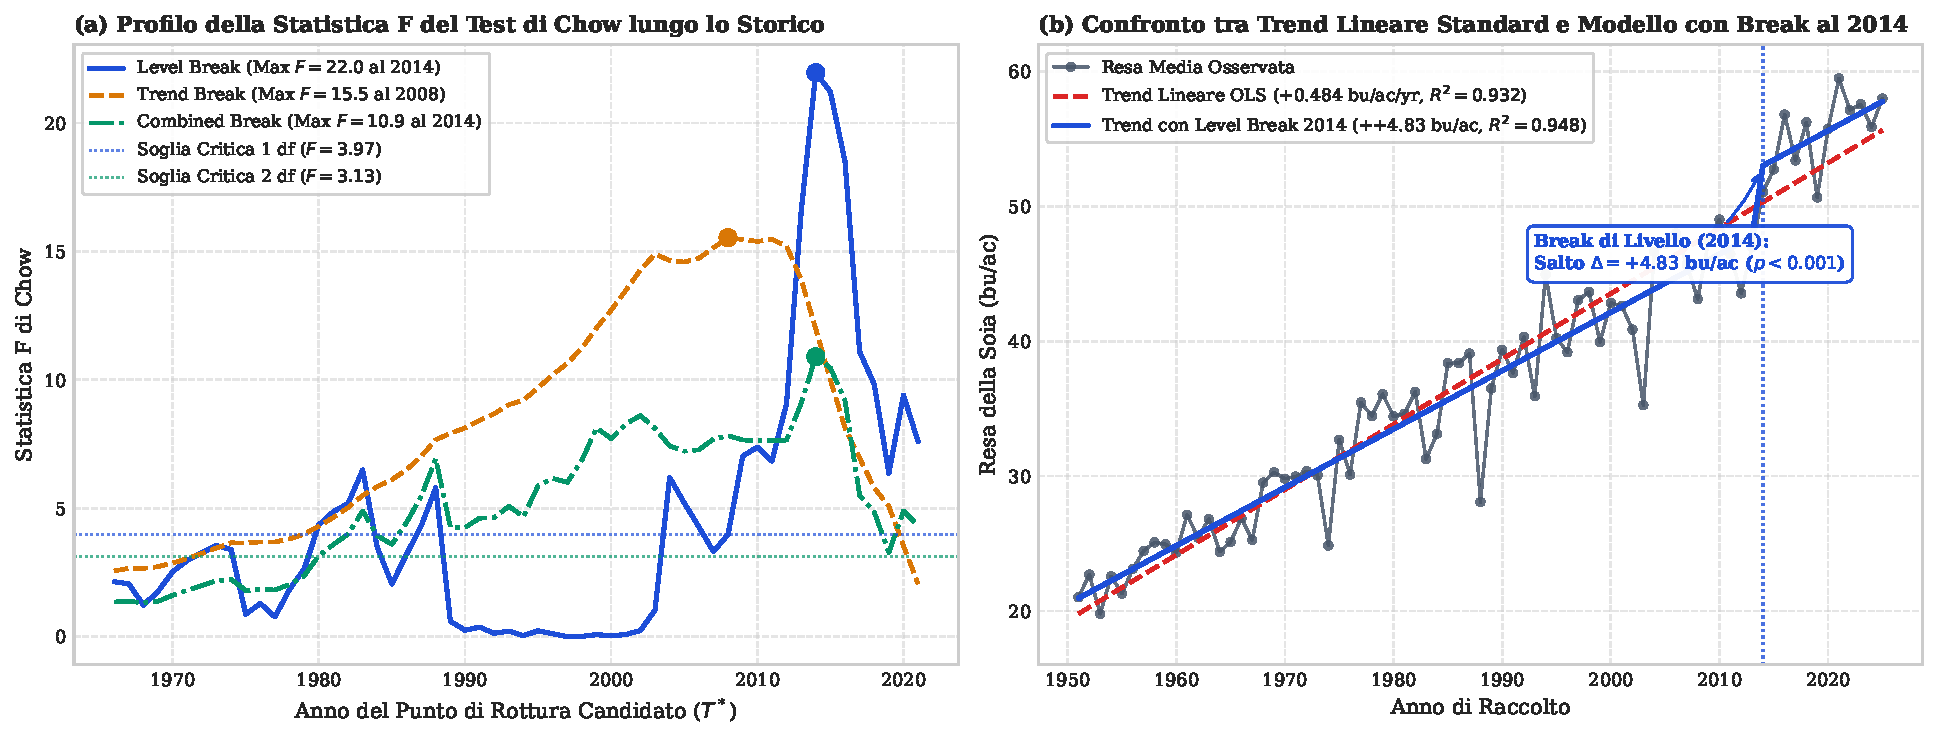
\includegraphics[width=0.92\textwidth]{figures/fig_chow_structural_break.pdf}
    \caption{Test di Chow per break strutturale (1951--2025): (a) statistica $F$ per anno candidato; (b) serie storica e salto di livello al 2014.}
    \label{fig:chow_break}
\end{figure}

\clearpage

% =============================================================================
% PAGINA 2: DISTRIBUZIONE ANOMALIE
% =============================================================================
\noindent \textbf{\large 3. Distribuzione delle anomalie di resa}
\vspace{0.15em}

\noindent Sull'intero storico (1951--2025), la distribuzione empirica delle anomalie presenta media nulla e deviazione standard di $4.67$\,bu/ac, con la caratteristica asimmetria negativa delle rese agricole ($44.0\%$ di anomalie negative; Tabella~\ref{tab:decile_distribution} e Figura~\ref{fig:decile_dist}). Nel periodo di test (2011--2025), mentre il trend expanding lineare sconta un'inerzia che sposta la media delle anomalie a $+2.41$\,bu/ac (riducendo le anomalie negative al $29.8\%$), il trend cubico mantiene la media centrata a $-0.06$\,bu/ac e la quota di anomalie negative al $44.7\%$, preservando la conformazione storica della coda sinistra.

\begin{table}[H]
\centering
\singlespacing
\scriptsize
\setlength{\tabcolsep}{3.5pt}
\renewcommand{\arraystretch}{1.06}
\caption{Distribuzione delle anomalie per decile: Trend Expanding vs Full-Sample (Cubico).}
\label{tab:decile_distribution}
\begin{tabular*}{\textwidth}{@{\extracolsep{\fill}} l cc cc @{}}
\toprule
& \multicolumn{2}{c}{\textbf{Trend Expanding (Baseline)}} & \multicolumn{2}{c}{\textbf{Trend Full-Sample (Oracolo Cubico)}} \\
\cmidrule(lr){2-3}\cmidrule(lr){4-5}
\textbf{Decile} & \textbf{Range} & \textbf{\% } $\epsilon < 0$ & \textbf{Range} & \textbf{\% } $\epsilon < 0$ \\
\midrule
\multicolumn{5}{l}{\textbf{Panel A: Intero Storico 1951--2025 ($N = 10{,}125$ osservazioni)}} \\
\midrule
$D_{1}$ (Crollo) & $[-25.5, -5.8]$ & 100\% & $[-25.1, -6.0]$ & 100\% \\
$D_{2}$ & $[-5.8, -3.2]$ & 100\% & $[-6.0, -3.3]$ & 100\% \\
$D_{3}$ & $[-3.2, -1.5]$ & 100\% & $[-3.3, -1.7]$ & 100\% \\
$D_{4}$ & $[-1.4, -0.2]$ & 100\% & $[-1.7, -0.5]$ & 100\% \\
$D_{5}$ & $[-0.2, +0.9]$ & 16\% & $[-0.5, +0.6]$ & 40\% \\
$D_{6}$ & $[+0.9, +1.9]$ & 0\% & $[+0.6, +1.6]$ & 0\% \\
$D_{7}$ & $[+1.9, +3.0]$ & 0\% & $[+1.6, +2.6]$ & 0\% \\
$D_{8}$ & $[+3.0, +4.3]$ & 0\% & $[+2.6, +3.7]$ & 0\% \\
$D_{9}$ & $[+4.3, +6.3]$ & 0\% & $[+3.7, +5.3]$ & 0\% \\
$D_{10}$ (Picco) & $[+6.3, +22.9]$ & 0\% & $[+5.3, +17.6]$ & 0\% \\
\midrule
\textbf{Totale} & $[-25.5, +22.9]$ & \textbf{41.6\%} & $[-25.1, +17.6]$ & \textbf{44.0\%} \\
\midrule[\heavyrulewidth]
\multicolumn{5}{l}{\textbf{Panel B: Periodo di Test Out-of-Sample 2011--2025 ($N = 2{,}025$ osservazioni)}} \\
\midrule
$D_{1}$ (Crollo) & $[-22.9, -5.2]$ & 100\% & $[-25.1, -6.9]$ & 100\% \\
$D_{2}$ & $[-5.2, -2.0]$ & 100\% & $[-6.9, -4.1]$ & 100\% \\
$D_{3}$ & $[-1.9, +0.0]$ & 98\% & $[-4.1, -2.2]$ & 100\% \\
$D_{4}$ & $[+0.0, +1.7]$ & 0\% & $[-2.1, -0.6]$ & 100\% \\
$D_{5}$ & $[+1.7, +3.1]$ & 0\% & $[-0.6, +0.6]$ & 47\% \\
$D_{6}$ & $[+3.2, +4.4]$ & 0\% & $[+0.7, +1.7]$ & 0\% \\
$D_{7}$ & $[+4.4, +5.6]$ & 0\% & $[+1.7, +2.9]$ & 0\% \\
$D_{8}$ & $[+5.6, +6.8]$ & 0\% & $[+2.9, +4.0]$ & 0\% \\
$D_{9}$ & $[+6.8, +8.8]$ & 0\% & $[+4.0, +5.6]$ & 0\% \\
$D_{10}$ (Picco) & $[+8.8, +22.9]$ & 0\% & $[+5.6, +17.6]$ & 0\% \\
\midrule
\textbf{Totale} & $[-22.9, +22.9]$ & \textbf{29.8\%} & $[-25.1, +17.6]$ & \textbf{44.7\%} \\
\bottomrule
\end{tabular*}
\end{table}

\begin{figure}[H]
    \centering
    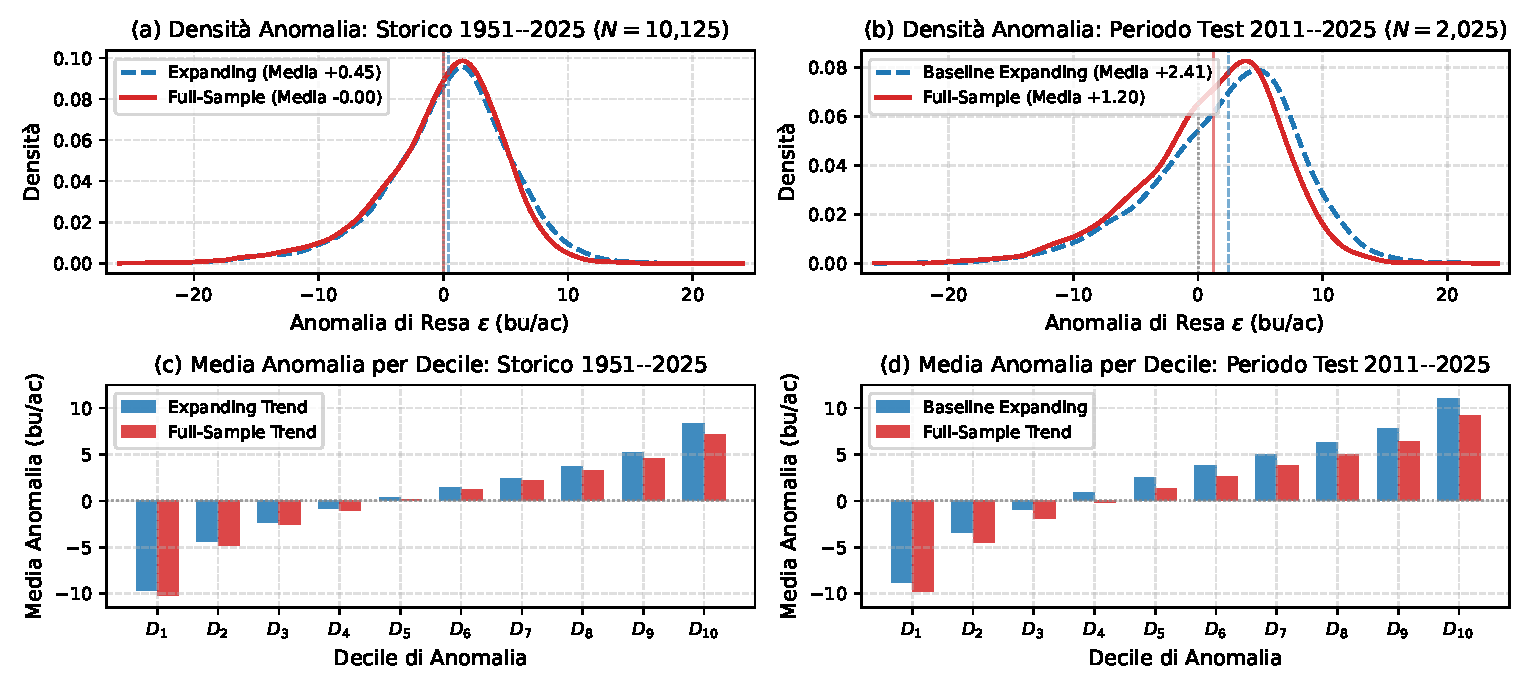
\includegraphics[width=0.88\textwidth]{figures/fig_decile_distribution_comparison.pdf}
    \caption{Distribuzione delle anomalie per decile: Baseline Expanding vs Full-Sample Cubico.}
    \label{fig:decile_dist}
\end{figure}

\clearpage

% =============================================================================
% PAGINA 3: CALIBRAZIONE DECILI ED ERRORE DI PREVISIONE (SHRINKAGE L2)
% =============================================================================
\noindent \textbf{\large 4. Errori di previsione e calibrazione per decile}
\vspace{0.15em}

\noindent L'analisi multi-orizzonte ($H=5$ fine giugno, $H=3$ fine agosto, $H=1^*$ chiusura raccolto; Tabella~\ref{tab:comp_decile_error_performance} e Figura~\ref{fig:decile_calibration_comp}) evidenzia due dinamiche distinte:
\begin{enumerate}
    \item \textbf{Miglioramento complessivo e sui decili centrali}: a chiusura raccolto ($H=1^*$), il trend cubico riduce l'errore medio assoluto tra decili osservati e previsti (MAE scende da $3.58$ a $2.92$\,bu/ac per la media modelli, con $r = 0.994$).
    \item \textbf{Persistenza della contrazione sul decile estremo ($D_1$)}: a fronte di un'anomalia osservata di $-10.18$\,bu/ac nel decile $D_1$ cubico, l'Ensemble prevede $-1.81$\,bu/ac (e la media modelli $-1.80$\,bu/ac), lasciando un residuo positivo di $+8.37$\,bu/ac, del tutto analogo a quello del trend expanding lineare (previsione di $-2.25$\,bu/ac su $-8.82$\,bu/ac osservati).
\end{enumerate}

\noindent Questo riscontro corrobora l'osservazione sui limiti dei decili incondizionati e conferma il ruolo della \textbf{contrazione $L_2$ (conditional shrinkage)}: poich\'e il meteo di contea spiega circa un terzo della varianza totale ($R^2 \approx 0.32$), la funzione di perdita quadratica contrae fisiologicamente le previsioni puntuali verso la media per non pagare pesanti scarti sul rumore locale non osservabile (grandine, drenaggio, parassiti). Lungo la stagione colturale, la previsione nel decile $D_1$ evolve coerentemente con l'accumulo del deficit estivo: prossima a zero a giugno ($H=5$), pari a $-1.62$\,bu/ac ad agosto ($H=3$) e $-1.81$\,bu/ac a fine ottobre ($H=1^*$).

\begin{table}[htbp]
\centering
\singlespacing
\footnotesize
\setlength{\tabcolsep}{3.2pt}
\renewcommand{\arraystretch}{1.08}
\caption{Decile mean point prediction ($\bar{\hat{\epsilon}}$, bu/ac) across realized yield anomaly deciles ($D_1 \dots D_{10}$) for key horizons ($H = 5, 3, 1^*$). Direct comparison between \textbf{Baseline} (Expanding Detrending) and \textbf{Full-Sample} (Oracle Trend).}
\label{tab:comp_decile_error_performance}
\begin{tabular*}{\textwidth}{@{\extracolsep{\fill}} l cc cc cc cc cc @{}}
\toprule
& \multicolumn{2}{c}{\textbf{Mean Observed}} & \multicolumn{2}{c}{\textbf{ElasticNet}} & \multicolumn{2}{c}{\textbf{Random Forest}} & \multicolumn{2}{c}{\textbf{XGBoost}} & \multicolumn{2}{c}{\textbf{LSTM (+Lag)}} \\
\cmidrule(lr){2-3}\cmidrule(lr){4-5}\cmidrule(lr){6-7}\cmidrule(lr){8-9}\cmidrule(lr){10-11}
\textbf{Decile} & \textbf{Base} & \textbf{Full} & \textbf{Base} & \textbf{Full} & \textbf{Base} & \textbf{Full} & \textbf{Base} & \textbf{Full} & \textbf{Base} & \textbf{Full} \\
\midrule
\multicolumn{11}{l}{\textbf{Panel A: Early Vegetative Horizon ($H=5$, June 30)}} \\
$D_{1}$ (Shortfall) & -8.82 & -9.81 & -1.69 & -2.54 & -1.78 & -2.48 & -2.08 & -3.15 & -0.98 & -0.86 \\
$D_{2}$ & -3.43 & -4.48 & -0.67 & -1.13 & -0.99 & -1.57 & -1.14 & -1.62 & -0.55 & -0.60 \\
$D_{3}$ & -0.93 & -1.87 & -0.26 & -0.75 & -0.57 & -1.13 & -0.46 & -1.08 & -0.17 & -0.28 \\
$D_{4}$ & +0.92 & -0.17 & +0.13 & -0.28 & -0.23 & -0.84 & +0.03 & -0.68 & +0.17 & +0.33 \\
$D_{5}$ & +2.48 & +1.29 & +0.26 & -0.11 & -0.14 & -0.35 & +0.04 & -0.31 & +0.36 & +0.11 \\
$D_{6}$ & +3.80 & +2.64 & +0.55 & +0.25 & +0.20 & -0.15 & +0.54 & -0.06 & +0.69 & +0.52 \\
$D_{7}$ & +5.02 & +3.83 & +0.67 & +0.19 & +0.32 & -0.09 & +0.72 & -0.01 & +0.58 & +0.79 \\
$D_{8}$ & +6.29 & +4.97 & +0.59 & +0.30 & +0.32 & +0.09 & +0.60 & +0.13 & +0.80 & +0.93 \\
$D_{9}$ & +7.77 & +6.37 & +1.01 & +0.23 & +0.60 & +0.07 & +0.84 & +0.06 & +1.19 & +0.67 \\
$D_{10}$ (Peak) & +11.01 & +9.23 & +0.77 & +0.58 & +0.18 & -0.06 & +0.37 & +0.07 & +0.79 & +0.15 \\
\midrule
\multicolumn{11}{l}{\textbf{Panel B: Pod-Filling Horizon ($H=3$, August 31)}} \\
$D_{1}$ (Shortfall) & -8.82 & -9.81 & -2.19 & -3.09 & -1.37 & -1.70 & -1.77 & -2.29 & -2.96 & -2.02 \\
$D_{2}$ & -3.43 & -4.48 & -0.84 & -1.33 & -0.59 & -1.00 & -0.59 & -1.14 & -1.26 & -0.90 \\
$D_{3}$ & -0.93 & -1.87 & -0.14 & -0.69 & -0.12 & -0.53 & -0.15 & -0.49 & -0.46 & -0.04 \\
$D_{4}$ & +0.92 & -0.17 & +0.56 & +0.20 & +0.34 & -0.04 & +0.73 & +0.18 & +0.43 & +0.45 \\
$D_{5}$ & +2.48 & +1.29 & +0.71 & +0.38 & +0.39 & +0.13 & +0.73 & +0.38 & +0.66 & +0.62 \\
$D_{6}$ & +3.80 & +2.64 & +1.11 & +0.86 & +0.68 & +0.48 & +1.23 & +0.81 & +1.18 & +1.36 \\
$D_{7}$ & +5.02 & +3.83 & +1.46 & +0.93 & +0.97 & +0.44 & +1.66 & +0.89 & +1.52 & +1.45 \\
$D_{8}$ & +6.29 & +4.97 & +1.56 & +1.32 & +1.01 & +0.90 & +1.72 & +1.40 & +1.56 & +1.64 \\
$D_{9}$ & +7.77 & +6.37 & +1.78 & +1.39 & +1.23 & +1.00 & +1.84 & +1.36 & +1.90 & +1.60 \\
$D_{10}$ (Peak) & +11.01 & +9.23 & +2.33 & +1.91 & +1.29 & +1.02 & +2.11 & +1.63 & +1.99 & +1.54 \\
\midrule
\multicolumn{11}{l}{\textbf{Panel C: Harvest Closure Horizon ($H=1^*$, October 31 / Sept 30 MN)}} \\
$D_{1}$ (Shortfall) & -8.82 & -9.81 & -2.13 & -3.17 & -1.49 & -1.94 & -1.59 & -2.26 & -3.08 & -2.93 \\
$D_{2}$ & -3.43 & -4.48 & -0.83 & -1.37 & -0.54 & -1.07 & -0.43 & -1.10 & -1.33 & -1.68 \\
$D_{3}$ & -0.93 & -1.87 & -0.24 & -0.80 & -0.18 & -0.57 & -0.19 & -0.51 & -0.39 & -0.94 \\
$D_{4}$ & +0.92 & -0.17 & +0.70 & +0.18 & +0.43 & -0.05 & +0.60 & +0.15 & +0.55 & -0.05 \\
$D_{5}$ & +2.48 & +1.29 & +1.05 & +0.50 & +0.51 & +0.13 & +0.84 & +0.33 & +0.67 & +0.20 \\
$D_{6}$ & +3.80 & +2.64 & +1.50 & +1.09 & +0.69 & +0.39 & +1.29 & +0.82 & +1.20 & +0.81 \\
$D_{7}$ & +5.02 & +3.83 & +1.84 & +1.20 & +1.14 & +0.50 & +1.86 & +1.00 & +1.50 & +0.80 \\
$D_{8}$ & +6.29 & +4.97 & +1.98 & +1.62 & +1.27 & +0.96 & +1.79 & +1.46 & +1.67 & +1.18 \\
$D_{9}$ & +7.77 & +6.37 & +2.21 & +1.67 & +1.36 & +0.92 & +2.01 & +1.52 & +2.05 & +1.22 \\
$D_{10}$ (Peak) & +11.01 & +9.23 & +2.86 & +2.25 & +1.61 & +1.12 & +2.33 & +1.82 & +2.24 & +1.09 \\
\bottomrule
\end{tabular*}
\vspace{0.2em}
{\footnotesize \textit{Source: Author's calculation on USDA NASS and ECMWF ERA5-Land data, 2011--2025 out-of-sample test evaluations ($2{,}025$ evaluations per horizon). Base: expanding-window trend; Full: whole-sample in-sample trend (1951--2025).}}
\end{table}

\begin{figure}[H]
    \centering
    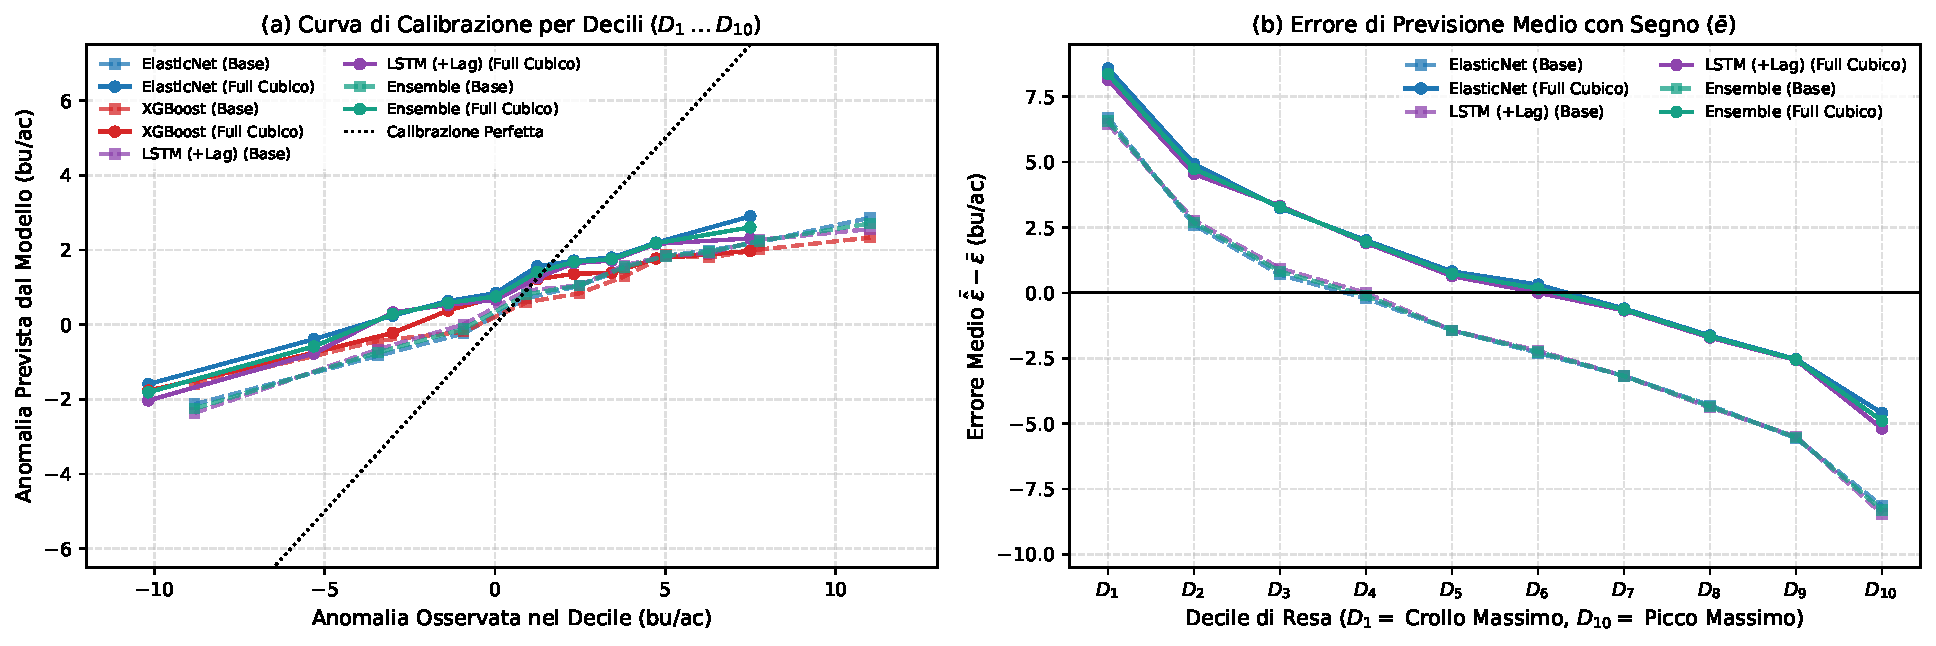
\includegraphics[width=0.82\textwidth]{figures/fig_decile_calibration_and_residuals_comparison.pdf}
    \caption{Calibrazione e residui per decile ($H=1^*$, 2011--2025): (a) osservato vs previsto; (b) errore medio con segno.}
    \label{fig:decile_calibration_comp}
\end{figure}

\clearpage

% =============================================================================
% PAGINA 4: RISOLUZIONE MACRO-REGIONALE E PROGRESSIONE MULTI-ORIZZONTE
% =============================================================================
\noindent \textbf{\large 5. Previsioni aggregate a livello regionale}
\vspace{0.15em}

\noindent Aggregando le previsioni sulle 135 contee, il rumore micro-climatico locale si compensa per la legge dei grandi numeri (Tabella~\ref{tab:yearly_raw_yields}). Per evitare ambiguit\`a dovute a scale di anomalia differenti tra i due trend, la tabella riporta direttamente le rese fisiche aggregate ($\bar{\hat{y}} = \bar{\tau} + \bar{\hat{\epsilon}}$), ordinando le annate per entit\`a dello shock rispetto al trend cubico ($\bar{\epsilon}_{\text{cub}}$):
\begin{itemize}
    \item Nello shock estremo del \textbf{2012} (resa reale $43.55$\,bu/ac, anomalia cubica $-5.56$\,bu/ac), mentre il trend secolare proietta un'annata normale errata ($47.62$\,bu/ac Base, $49.11$\,bu/ac Cubico), l'Ensemble stima $43.53$\,bu/ac (Base, errore $-0.02$) e \textbf{$43.71$\,bu/ac} (Cubico, errore $+0.16$).
    \item Su tutti i 15 anni di test, il trend cubico azzera il bias secolare (Bias $+0.06$\,bu/ac vs $-2.41$\,bu/ac) e riduce il MAE dell'Ensemble da $1.87$ a \textbf{$1.46$\,bu/ac} ($1.40$\,bu/ac per la media modelli).
\end{itemize}

\begin{table}[H]
\centering
\singlespacing
\scriptsize
\setlength{\tabcolsep}{1.8pt}
\renewcommand{\arraystretch}{1.06}
\caption{Previsioni regionali aggregate di resa ($\bar{\hat{y}}$, bu/ac) a chiusura raccolto ($H = 1^*$) sui 15 anni di test ordinati per discostamento dal trend cubico. Tra parentesi l'anomalia cubica reale ($\bar{\epsilon}_{\text{cub}}$). In grassetto il valore pi\`u vicino al dato reale.}
\label{tab:yearly_raw_yields}
\begin{tabular*}{\textwidth}{@{\extracolsep{\fill}} c c cc cc cc cc cc cc @{}}
\toprule
& & \multicolumn{2}{c}{\textbf{Secular } $\bar{\tau}$} & \multicolumn{2}{c}{\textbf{ElasticNet}} & \multicolumn{2}{c}{\textbf{XGBoost}} & \multicolumn{2}{c}{\textbf{LSTM (+Lag)}} & \multicolumn{2}{c}{\textbf{Ensemble}} & \multicolumn{2}{c}{\textbf{Media Modelli}} \\
\cmidrule(lr){3-4}\cmidrule(lr){5-6}\cmidrule(lr){7-8}\cmidrule(lr){9-10}\cmidrule(lr){11-12}\cmidrule(lr){13-14}
\textbf{Anno} & \textbf{Reale ($\bar{\epsilon}_{\text{cub}}$)} & \textbf{Base} & \textbf{Full} & \textbf{Base} & \textbf{Full} & \textbf{Base} & \textbf{Full} & \textbf{Base} & \textbf{Full} & \textbf{Base} & \textbf{Full} & \textbf{Base} & \textbf{Full} \\
\midrule
2012 & 43.55 {\tiny (-5.56)} & \textbf{47.62} & 49.11 & \textbf{43.80} & 46.23 & \textbf{44.69} & 45.64 & \textbf{43.26} & 41.20 & \textbf{43.53} & 43.71 & \textbf{43.82} & 44.20 \\
2019 & 50.66 {\tiny (-3.46)} & \textbf{51.75} & 54.12 & \textbf{52.74} & 55.46 & \textbf{51.50} & 54.15 & \textbf{52.30} & 54.64 & \textbf{52.52} & 55.05 & \textbf{52.27} & 54.82 \\
2013 & 46.99 {\tiny (-2.78)} & \textbf{47.79} & 49.78 & 45.33 & \textbf{47.42} & 45.58 & \textbf{47.80} & 45.69 & \textbf{48.26} & 45.51 & \textbf{47.84} & 45.53 & \textbf{47.83} \\
2024 & 55.89 {\tiny (-2.34)} & \textbf{54.98} & 58.23 & \textbf{57.85} & 60.35 & \textbf{57.31} & 59.98 & \textbf{55.69} & 60.70 & \textbf{56.77} & 60.52 & \textbf{56.90} & 60.39 \\
2011 & 46.47 {\tiny (-1.99)} & \textbf{47.23} & 48.46 & \textbf{46.34} & 47.95 & 45.69 & \textbf{46.89} & \textbf{45.60} & 48.41 & \textbf{45.97} & 48.18 & \textbf{45.90} & 47.86 \\
2025 & 58.00 {\tiny (-1.11)} & 55.51 & \textbf{59.11} & 55.36 & \textbf{60.20} & \textbf{56.13} & 60.10 & \textbf{56.70} & 60.33 & \textbf{56.03} & 60.27 & \textbf{56.06} & 60.23 \\
2023 & 57.57 {\tiny (+0.21)} & 54.33 & \textbf{57.37} & 55.97 & \textbf{59.00} & 55.93 & \textbf{58.66} & 55.11 & \textbf{58.19} & 55.54 & \textbf{58.59} & 55.64 & \textbf{58.61} \\
2014 & 51.06 {\tiny (+0.60)} & 48.18 & \textbf{50.46} & 47.62 & \textbf{49.44} & 49.83 & \textbf{51.30} & 49.62 & \textbf{51.61} & 48.62 & \textbf{50.52} & 48.92 & \textbf{50.72} \\
2022 & 57.14 {\tiny (+0.61)} & 53.66 & \textbf{56.53} & 53.85 & \textbf{55.77} & 54.94 & \textbf{57.44} & 55.86 & \textbf{58.16} & 54.86 & \textbf{56.97} & 54.88 & \textbf{57.09} \\
2017 & 53.41 {\tiny (+0.81)} & 50.35 & \textbf{52.60} & \textbf{53.57} & 55.78 & 52.36 & \textbf{54.31} & \textbf{52.18} & 54.94 & \textbf{52.88} & 55.36 & \textbf{52.75} & 55.10 \\
2020 & 55.75 {\tiny (+0.85)} & 52.15 & \textbf{54.90} & 52.99 & \textbf{55.86} & 52.99 & \textbf{55.64} & 54.33 & \textbf{54.89} & 53.66 & \textbf{55.38} & 53.49 & \textbf{55.44} \\
2015 & 52.74 {\tiny (+1.58)} & 48.79 & \textbf{51.16} & 50.64 & \textbf{52.83} & 50.77 & \textbf{52.47} & 51.21 & \textbf{53.95} & 50.92 & \textbf{53.39} & 50.88 & \textbf{53.16} \\
2018 & 56.23 {\tiny (+2.88)} & 50.99 & \textbf{53.35} & 53.75 & \textbf{56.85} & 53.54 & \textbf{55.61} & 53.82 & \textbf{56.45} & 53.79 & \textbf{56.65} & 53.73 & \textbf{56.39} \\
2021 & 59.50 {\tiny (+3.79)} & 52.82 & \textbf{55.70} & 55.67 & \textbf{58.59} & 54.74 & \textbf{57.54} & 55.45 & \textbf{58.00} & 55.56 & \textbf{58.30} & 55.35 & \textbf{58.11} \\
2016 & 56.81 {\tiny (+4.94)} & 49.47 & \textbf{51.87} & 53.56 & \textbf{55.82} & 52.35 & \textbf{54.30} & 52.41 & \textbf{54.68} & 52.99 & \textbf{55.25} & 52.83 & \textbf{55.01} \\
\midrule
\textbf{Bias Medio} & --- & -2.41 & \textbf{+0.06} & -1.52 & \textbf{+1.05} & -1.56 & \textbf{+0.67} & -1.50 & \textbf{+0.84} & -1.51 & \textbf{+0.95} & -1.52 & \textbf{+0.88} \\
\textbf{MAE} & --- & 3.31 & \textbf{2.24} & 2.11 & \textbf{1.70} & 2.02 & \textbf{1.40} & \textbf{1.72} & 1.75 & 1.87 & \textbf{1.46} & 1.91 & \textbf{1.40} \\
\textbf{RMSE} & --- & 3.84 & \textbf{2.75} & 2.40 & \textbf{2.19} & 2.33 & \textbf{1.85} & \textbf{2.07} & 2.14 & 2.16 & \textbf{1.99} & 2.19 & \textbf{1.92} \\
\textbf{Pearson } $r$ & --- & 0.789 & \textbf{0.811} & \textbf{0.915} & 0.912 & \textbf{0.933} & 0.928 & \textbf{0.955} & 0.920 & \textbf{0.946} & 0.930 & \textbf{0.945} & 0.932 \\
\bottomrule
\end{tabular*}
\end{table}

\vspace{0.35em}
% -----------------------------------------------------------------------------
% 6. PROGRESSIONE MULTI-ORIZZONTE
% -----------------------------------------------------------------------------
\noindent \textbf{\large 6. Andamento lungo gli orizzonti previsivi}
\vspace{0.15em}

\noindent Anche guardando l'evoluzione mese per mese durante la stagione (Figura~\ref{fig:r2_progression_comp}), il comportamento e la gerarchia dei modelli non cambiano tra i due trend: il segnale meteo compare ad agosto ($H=3$) e i modelli migliori restano stabilmente l'Ensemble e l'LSTM.

\begin{figure}[H]
    \centering
    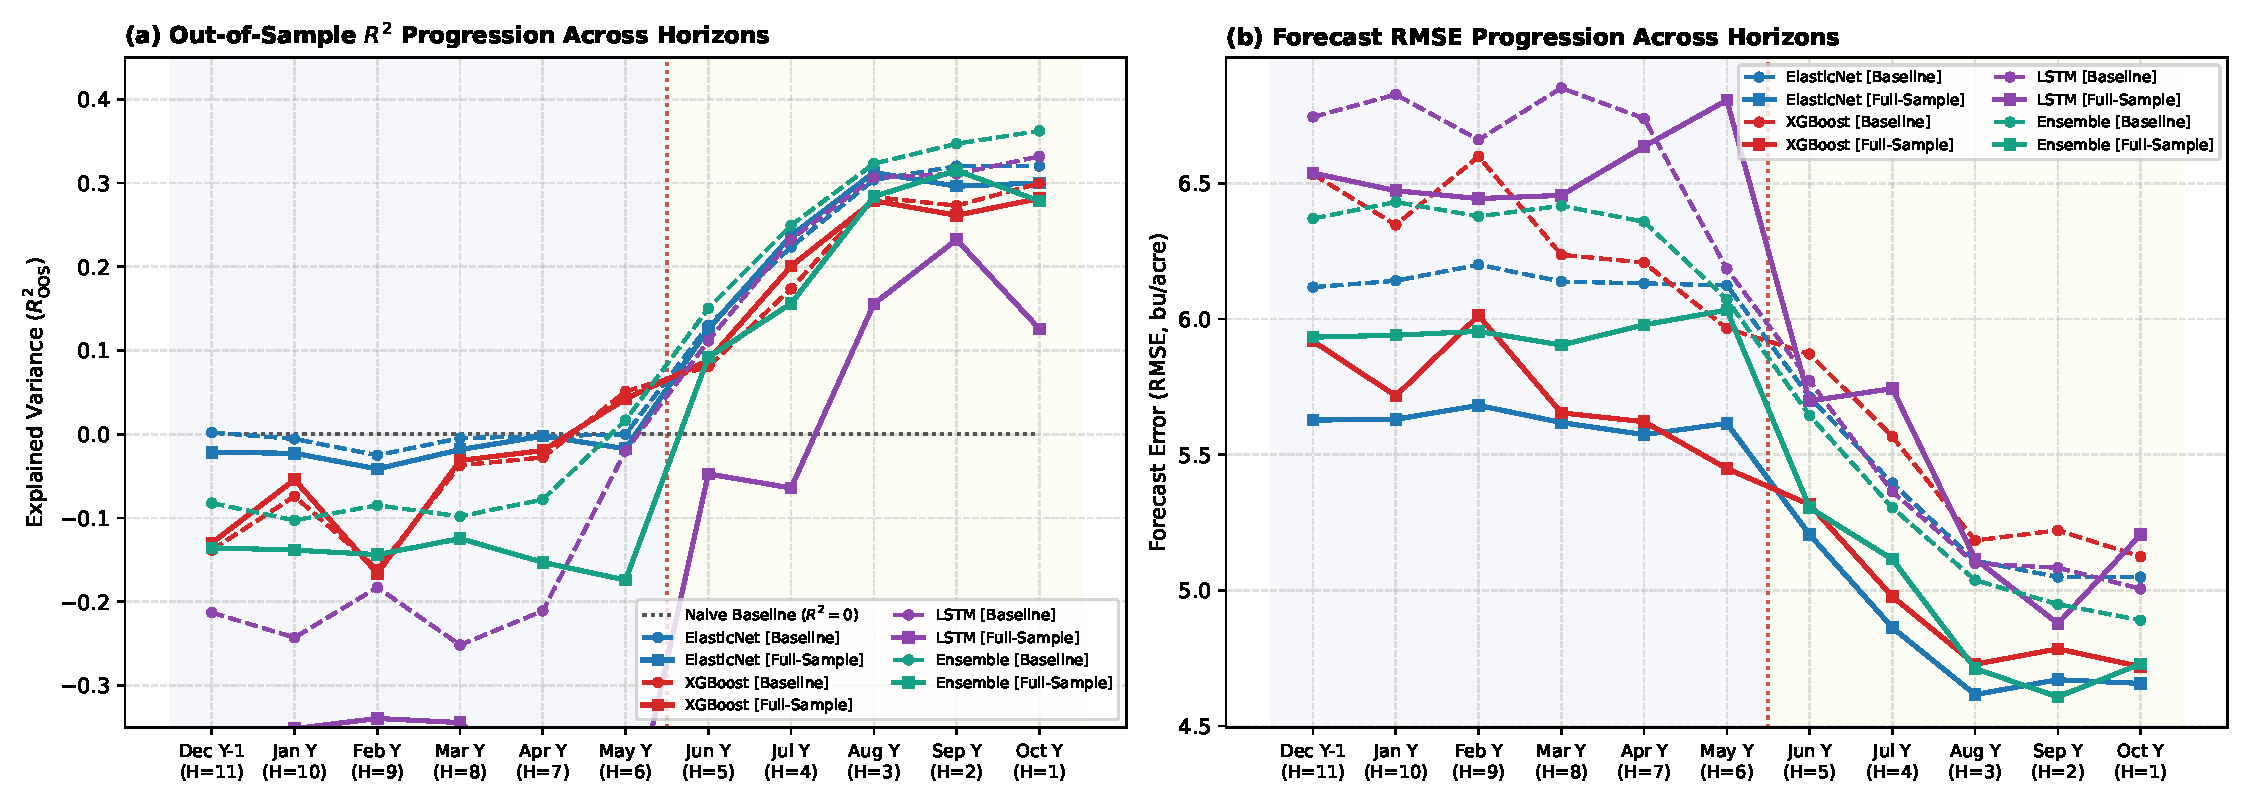
\includegraphics[width=0.82\textwidth]{figures/fig_r2_horizon_progression_comparison.pdf}
    \caption{Progressione delle performance lungo gli orizzonti previsivi ($H=11 \dots 1$): $R^2_{\text{OOS}}$ e RMSE (2011--2025).}
    \label{fig:r2_progression_comp}
\end{figure}

\end{document}
